\documentclass[11pt]{article}
\usepackage{geometry, titlesec}
\usepackage[parfill]{parskip}
\usepackage[italicdiff]{physics}
\usepackage{amsfonts, amsthm}
\usepackage[cm]{fullpage}
\usepackage{fancyhdr}
\usepackage{enumitem}
\usepackage{xcolor, soul}
\usepackage{graphicx}
\usepackage{siunitx}
%\allowdisplaybreaks

\renewcommand{\thesubsection}{\thesection.\alph{subsection}}
\setenumerate[1]{label={(\alph*)}}

\makeatletter
\renewcommand*\env@cases[1][1.2]{%
  \let\@ifnextchar\new@ifnextchar
  \left\lbrace
  \def\arraystretch{#1}%
  \array{@{}l@{\quad}l@{}}%
}
\makeatother
 
\renewcommand{\footrulewidth}{.2pt}
%\setlist[enumerate]{leftmargin=*}
\pagestyle{fancy}
\fancyhf{}
\lhead{Physics 132-B}
\chead{\textbf{Discussion 2 Problems}}
\rhead{A--De Discussion}
\setlength{\headheight}{11pt}
\setlength{\headsep}{11pt}
\setlength{\footskip}{24pt}
\lfoot{\today}
\rfoot{\thepage}

\titleformat{\subsection}[runin]{\normalfont\large\bfseries}{\thesubsection}{1em}{}
\newcommand{\refeq}[1]{(\ref{#1})}

\newcommand{\beq}{\begin{equation*}}
\newcommand{\eeq}{\end{equation*}}

\newcommand{\beqn}{\begin{equation}}
\newcommand{\eeqn}{\end{equation}}

\newcommand{\blg}{\begin{align*}}
\newcommand{\elg}{\end{align*}}


\newenvironment{statement}
{
%    \color{gray}
    \ignorespaces
}
{
%    \smallskip
}

\newenvironment{problem}
{
    \color{darkgray}
    \ignorespaces
}

\newenvironment{solution}
{
    \paragraph{Solution.}
    \ignorespaces
}
{
    \bigskip
}

\renewcommand{\vec}[1]{\mathbf{#1}}
\newcommand{\imgscale}{1.7}

\addtolength{\tabcolsep}{.2in}

\begin{document}

%\begin{tabular}{c c c}
%	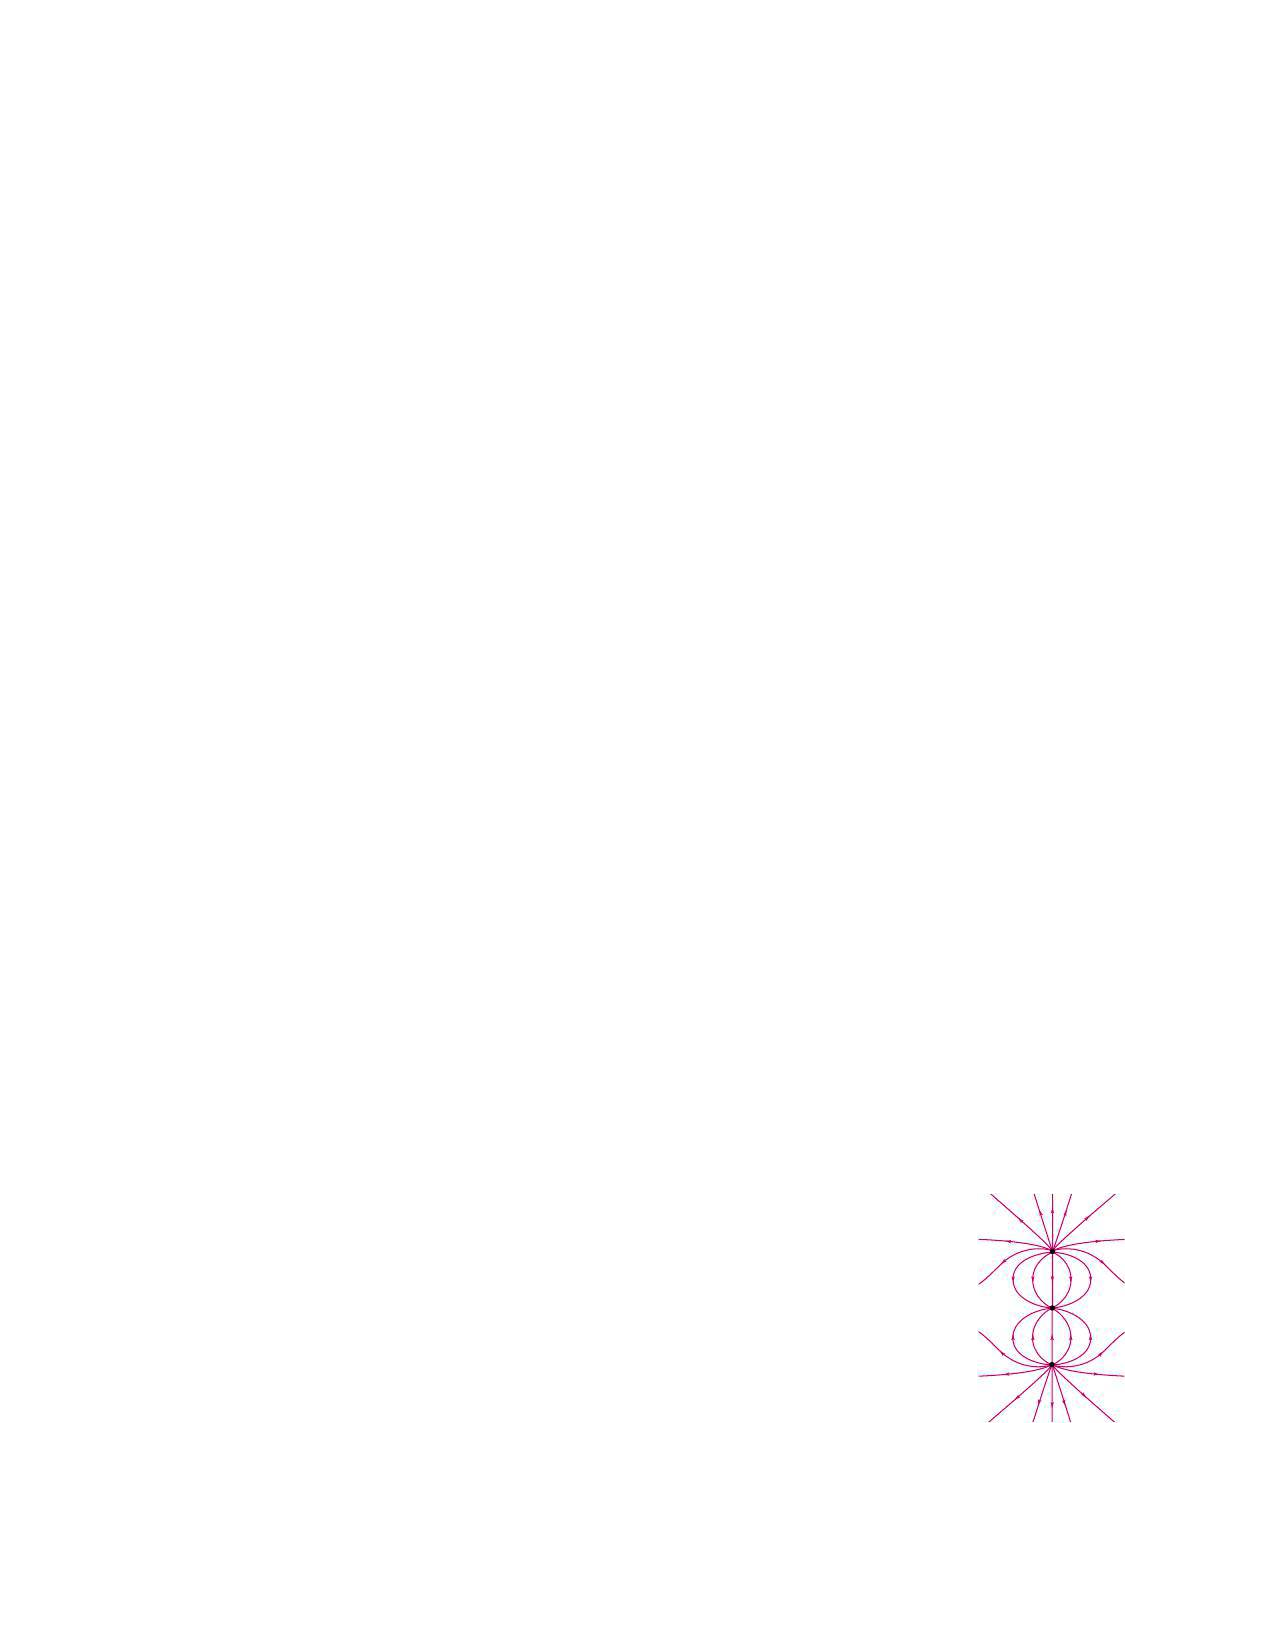
\includegraphics[scale=\imgscale]{Q21-7} & 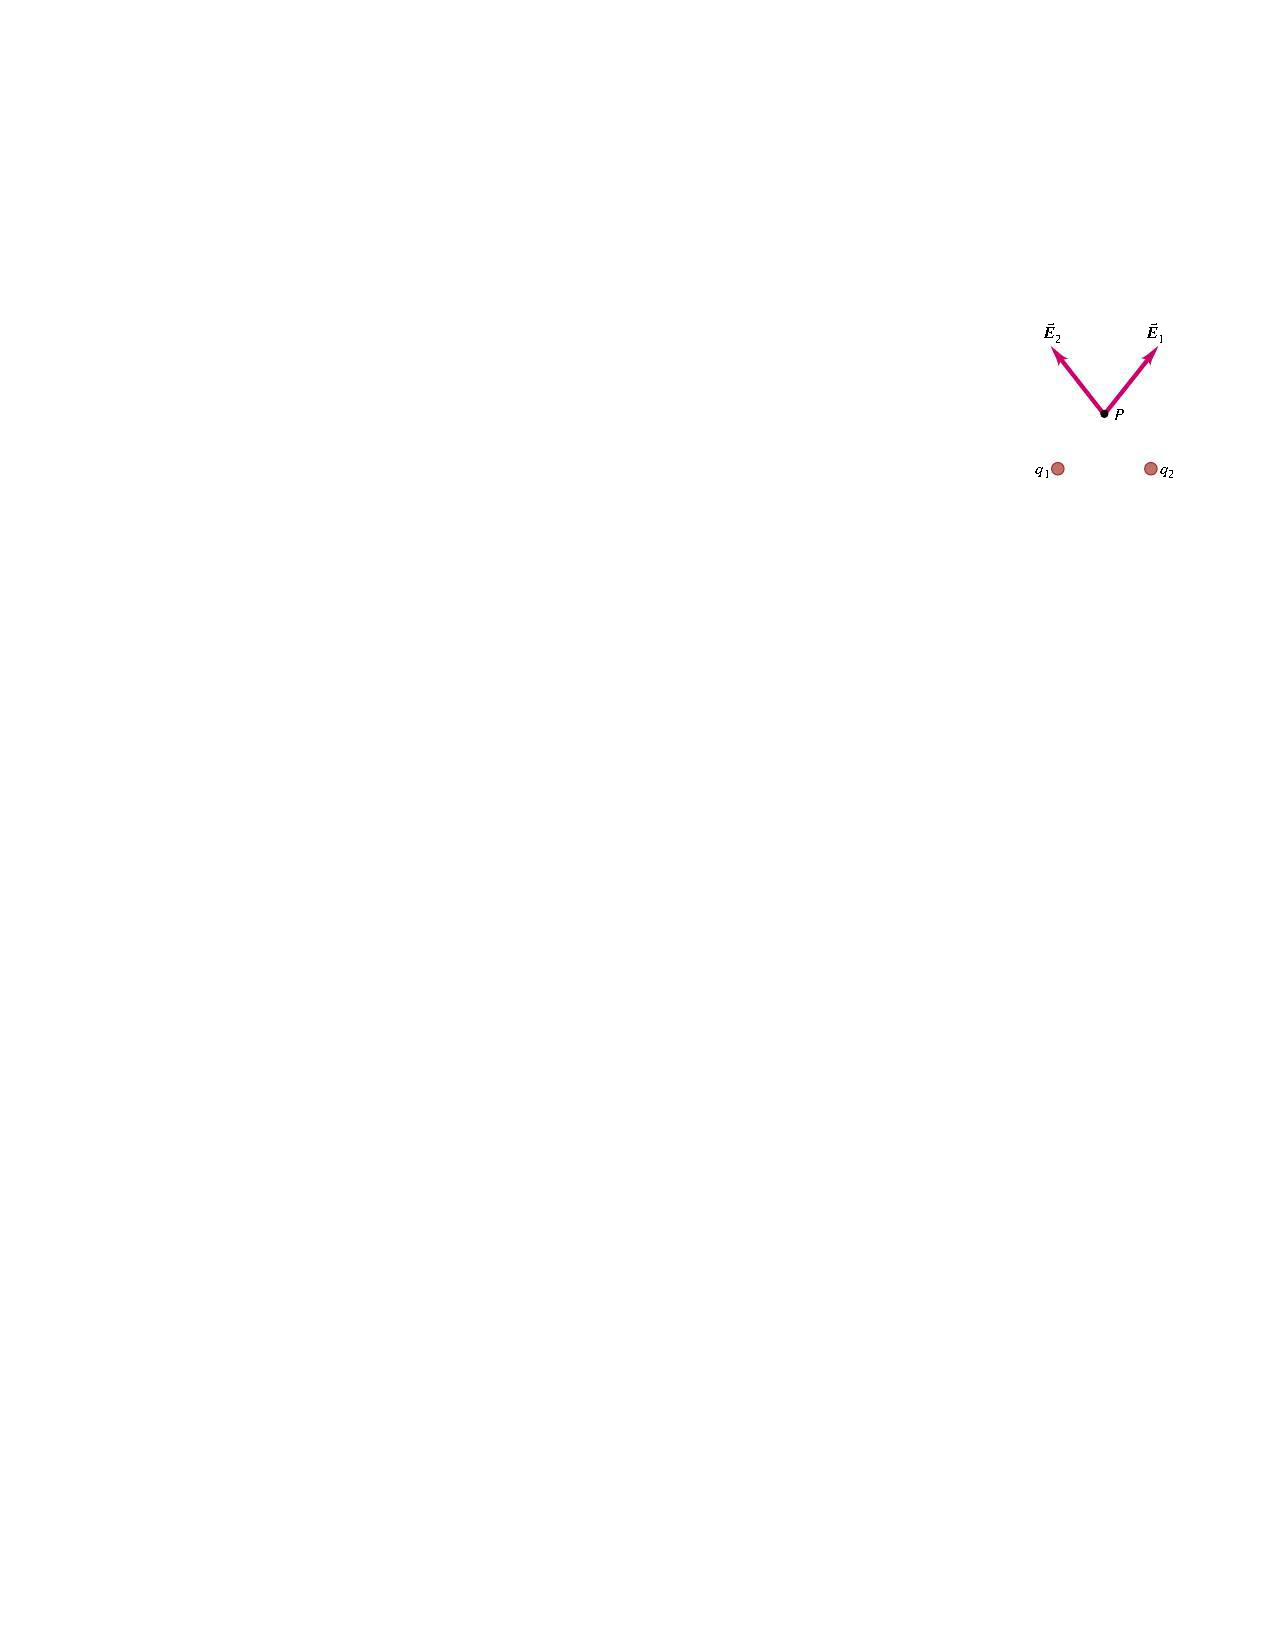
\includegraphics[scale=\imgscale]{Q21-22} & 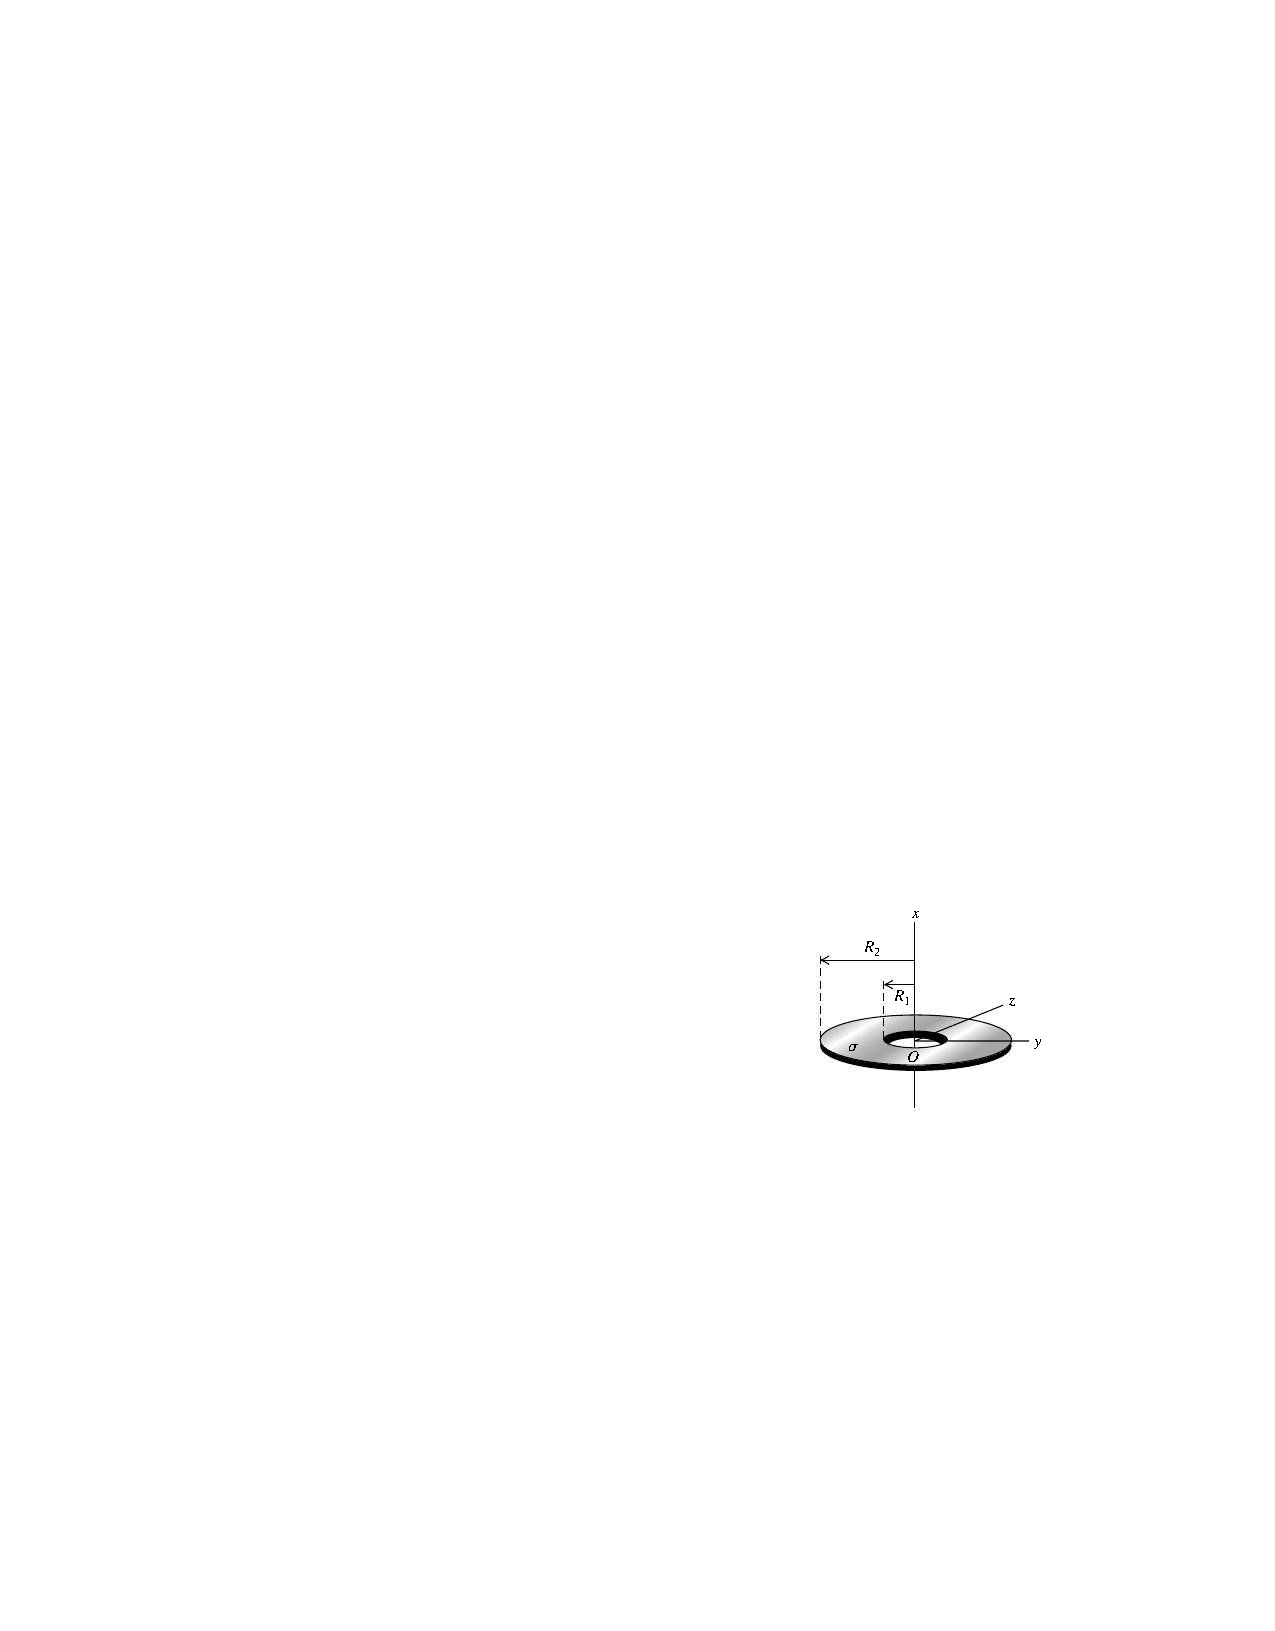
\includegraphics[scale=\imgscale]{P21-87} \\
%	\textbf{Figure Q21.7} & \textbf{Figure Q21.22} & \textbf{Figure P21.87} \\
%\end{tabular}
	

\newcommand{\vE}{\vec{E}}

\paragraph{Question 22.5}
\begin{problem}
	A spherical Gaussian surface encloses a point charge $q$.  If the point charge is moved from the center of the sphere to a point away from the center, does the electric field at a point on the surface change?  Does the total flux through the Gaussian surface change?  Explain.
\end{problem}

\vfill

\paragraph{Question 22.14}
\begin{problem}
	In a certain region of space, the electric field $\vE$ is uniform.
	\begin{enumerate}
		\item Use Gauss's law to prove that this region of space must be electrically neutral; that is, the volume charge density $\rho$ must be zero.
		\item Is the converse true?  That is, in a region of space where there is no charge, must $\vE$ be uniform?  Explain.
	\end{enumerate}
\end{problem}

\vfill

\paragraph{Question 22.15}
\begin{problem}
	\begin{enumerate}
		\item In a certain region of space, the volume charge density $\rho$ has a uniform positive value.  Can $\vE$ be uniform in this region?  Explain.
		\item Suppose that in this region of uniform positive $\rho$ there is a ``bubble'' within which $\rho = 0$.  Can $\vE$ be uniform within this bubble?  Explain.
	\end{enumerate}
\end{problem}

\vfill

\clearpage

\paragraph{Problem 22.62}
\begin{problem}
	A region in space contains a total positive charge $Q$ that is distributed spherically such that the volume charge density $\rho(r)$ is given by
	\begin{align*}
		\rho(r) &= \frac{3 \alpha r}{2 R} \quad\text{for } r \leq \frac{R}{2}, &
		\rho(r) &= \alpha \left[ 1 - \left( \frac{r}{R} \right)^2 \right] \quad\text{for } \frac{R}{2} \leq r \leq R, &
		\rho(r) &= 0 \quad\text{for } r \geq R.
	\end{align*}
	Here $\alpha$ is a positive constant having units of \si{\coulomb\per\cubic\meter}.
	\begin{enumerate}
		\item Determine $\alpha$ in terms of $Q$ and $R$.
		\item Using Gauss's law, derive an expression for the magnitude of the electric field as a function of $r$.  Do this separately for all three regions.  Express your answers in terms of $Q$.
		\item What fraction of the total charge is contained within the region $R/2 \leq r \leq R$?
		\item What is the magnitude of $\vE$ at $r = R / 2$?
	\end{enumerate}
\end{problem}

\end{document}